\chapter{Аналитический раздел}
\label{cha:analysis}

Выделение голосовой составляющей из аудио сигнала является частным случаем задачи разделения комбинации аудио сигналов на составляющие. Музыкальное произведение может быть записано как с использованием нескольких микрофонов, захватывающих разные источники, при этом изоляция источников будет ограничена, либо с использованием выделенной на каждый источник. Все записанные сигналы в последствии проходят процесс сведения для получения итоговой аудио записи. Тем самым конечный аудио сигнал можно представить в виде суммы отдельных источников с приминением фильтров к каждому источнику.

Математически это можно записать как:

\begin{equation}
 x(t) = \sum_{j=1}^{J} \sum_{\tau=-\infty}^{\infty} a_{j}(t-\tau, \tau)s_j(t-\tau)
 \label{anal:result-signal}
\end{equation}

где 

\begin{itemize}
	\item $x$ -- итоговый аудио сигнал;
	\item $s_j$ -- сигнал источника;
	\item $J$ -- количество источников;
	\item $a_j$ -- фильтр, примененный к источнику в процессе сведения.
\end{itemize}

Если приминяемые фильтры являются линейными, то итоговый сигнал представляет собой линейную комбинацию. С другой стороны, к итоговому сигналу так же могут быть применены фильтры. С этой точки зрения сведенный сигнал перестает быть линейной суммой отдельных источников. 

Тем самым, итоговая запись, в контексте задачи выделения аудио источников, может быть определена по следующим признакам\cite{[Chandna}:

\begin{enumerate}
	\item Количество используемых во время записи источников аудио сигнала. Источники могут быть записаны как отдельно, с помощью выделенных линий звукозаписи либо нескольких микровонов, так и при помощи одного микрофона, захватывающего все звуки одновременно. С понижением количества звукозаписывающих устройств повышается смешанность отдельных аудио сигналов и влияние на них шумов.
	\item Количество примененных к итоговому аудио сигналу эффектов. С учетом итоговых фильтров формула \ref{anal:result-signal} принимает вид:
	\begin{equation}
	x(t) =\prod_{k=1}^K \psi_{k}(t) \sum_{j=1}^{J} \sum_{\tau=-\infty}^{\infty} a_{j}(t-\tau, \tau)s_j(t-\tau)
	\label{anal:filtered-signal}
	\end{equation}
	где $\psi_{k}(t), k=1б ..., K$ -- применяемые к итоговому сигналу фильтры.
	Исходя из формулы, применение фильтров к итоговому сигналу усложняет задачу выделения аудио источников.
	\item Изменение положения звукозаписывающих устройств во время записи. Микрофоны, ведущие запись, могут быть статичными, находясь в закрепленном состоянии, либо перемещаться, например от одного источника к другому. Второй случай оказывает непосредственное влияние на сигналы аудио источников, добавляя шумы и изменяя уровень сигнала.
\end{enumerate}

Эта работа будет сфокусирована на обработке записей без итоговых фильтров, источники которых были записаны независимо друг от друга без изменений положения звукозаписывающих устройств.

\section{Цифровое представление аудио сигналов}

Звук имеет три основных характеритичесих параметров: амплитуда, частота и фаза. Две последнии характеристики являются функциями времени, в то время как амплитуда определяет динамический диапозон. По этому в цифровом представлении аудио сигнала записываются изменения аплитуды как функция времени. Тем самым процесс отцифровки аналогового аудио сигнала является записью мгновенных амплитудных значений (дискретизация по амплитуда) в постоянные моменты времени (дискретизация по времени). Графическое представление дискретизации аналогового сигнала представлено на рисунке \ref{anal:atob}.

\begin{figure}
	\centering
	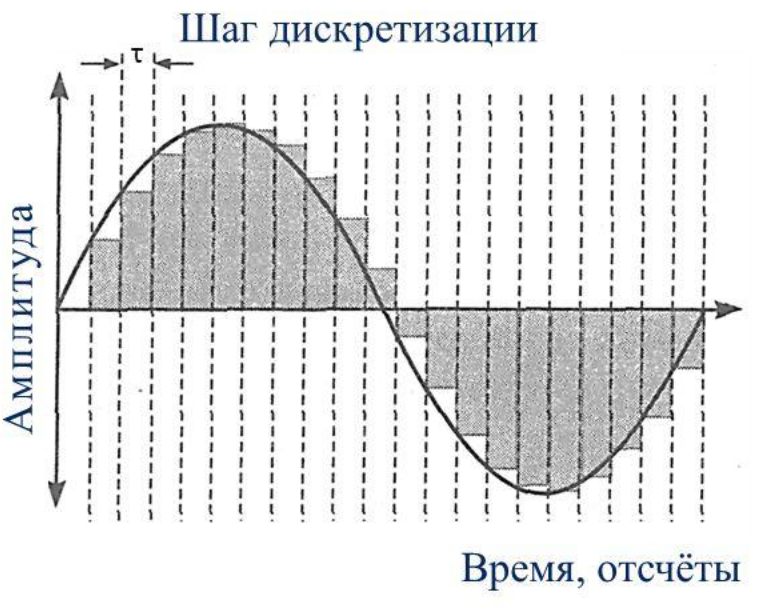
\includegraphics[width=0.5\textwidth]{inc/img/analog-to-bin.png}
	\caption{Дискретизация аналогового сигнала}
	\label{anal:atob}
\end{figure}

Для определения периода записи амплитудных значений задается частота дискретизации. 

Существует теорема Котельникова\cite{Bikkenin}, утверждающая, что <<любую функцию $F(t)$, состоящую из частот от 0 до $f_1$, можно непрерывно передавать с любой точностью при помощи чисел, следующих друг за другом через $1/(2f_1)$ секунд>>.

При максимальной воспринимаемой человеческим ухом частоте в 20 кГц, по теореме Котельникова минимальная необходимая частота дискретизации должна быть 40 кГц.

Стандартная частота дискретизации аудио сигнала составляет 44,1 кГц, максимальная -- 192 кГц.

Для определения максимального значения амплитуды используется значение квантования (или разрядность), задающаяся в битах. В зависимости от используемого формата разрядность может быть 1, 8, 16, 24 и 32 бит.

В данной работе будут использоваться wav-файлы (сокращение Waveform Audio File Format). Формат WAVE был разработан корпорацией Майкрософт, является контейнером для хранения и записи оцифрованных аудиопотоков. Представляет из себя сжатый формат, отличается отсутствием потери качества и основан на расширении RIFF. Структура wav-файлов имеет чёткую форму, описанную в стандарте \cite{wav}.

\section{Существующие методы выделения источников}

Методы выделения источников делятся на две основные категории\cite{mansour:hal-00802445}.

\begin{itemize}
	\item Слепое выделение. Методы, относяющиеся к данной категории, обрабатывают смесь аудио сигналов без помощи, или с минимальным количеством, информации об источниках и методах их сведения. Наиболее популярные из этих алгоритмов используют (предполагаемую) статистическую независимость исходных сигналов. Примером являются Метод главных компонент \cite{Lopez} \cite{Dadula}, Факторизация неотрицательных матриц. С ростом количества исследований в области нейронных сетей возникла идея применения методов глубинного обучения в задачах выделения источников. Работы по данной теме были сфокусированы на таких сетях как Глубинные и Сверточные нейронные сети.
	\item Информированное выделение. Для данной категории методов предполагается наличие предварительной информации об исходных сигналах, в форме MIDI, партитуры или другом виде представления музыки\cite{Miron}. Целью данной работы не является изучение информированного выделения, потому детального описания представлено не будет.
\end{itemize}

Данная работа будет сфокусирована на методах слепого выделения.

\subsection{Метод главных компонент}
Метод главных компонент (англ. Principal Component Analysis) и анализ независимых компонент (англ. Independent Component Analysis) -- это статистические способы уменьшения размерности данных, который являлся объектом для исследований в области выделения аудио источников \cite{Lopez} \cite{Dadula}.

Основная идея этоих метода заключается в том, чтобы проецировать данные из временных рядов, таких как аудиозапись, в новые системы отсчета, которые основаны на некотором статистическом критерии. Эти оси являются статистически независимые в отличие от преобразования Фурье, где данные временной области проецируются на оси частот, которые могут перекрываться. Частотные оси в преобразовании Фурье остаются неизменными независимо от анализируемой части, тогда как в методе главных компонент и анализе независимых компонент оси являются динамическими и различны для каждой анализируемой части. После нахождения, оси, на которые происходит проецирование, могут быть разделены и инвертированы для нахождения источников, представленных в исходном сигнале.

Формулу \ref{anal:result-signal} можно представить в виде:

\begin{equation}
x(t) = As(t)
\end{equation}

где

\begin{itemize}
	\item $A$ -- квадратная матрица, состоящая из коэффициентов исходного сигнала.
	\item $s(t)$ -- множество сигналов выделяемых источников.
\end{itemize}

Имея оценку матрицы $A$ можно получить искомые источники с помощью обратной ей матрицы $W$:

\begin{equation}
y(t) = Wx(t)
\end{equation}

В рамках задачи слепого выделения источников данный метод сводится к серии матричных произведений, представляющих свобой фильтры. В общем случае входной сигнал $X$ размерности $N$ из $M$ образцов (представляется матрицей размерности $NxM$) может быть приведен к сигналу $Y$ с использованием матрицы преобразования $W$ размерности $NxN$ как $Y^T = WX^T$. Такое преобразование проецирует сигнал на разные оси основываясь на матрице преобразования. Если размер полученного сигнала равен размер исходного сигнала, то преобразование называется ортогональным и оси перпендикулярны.

Данный метод является иттеративным с фиксированной точкой. В нем применяется нелиейная функция $g(y) = th(a * y)$, которая применяется к матрице разделения $W$, которая пересчитывается на каждом шаге.

Входные данные для данного метода должны быть обработаны следующей последовательностью действий:

\begin{enumerate}
	\item центрирование по среднему значению;
	\item нормализация по дисперсии;
	\item ортоганализация.
\end{enumerate}

После этого случайным образом выбирается начальное значение вектора $W$, которое уточняется с помощью следующих иттеративных шагов:

\begin{enumerate}
	\item Обновление $W$ по формуле:
	
	\begin{equation}
		w = E\{zg(w^Tz)\} - E\{g'(w^Tz)\}w
	\end{equation}
	
	где $z$ -- обработанные входные данные.
	\item $w = \frac{w}{|| w ||}$
\end{enumerate}

Выполняются до достижения сходимости.

\subsection{Факторизация неотрицательных матриц}

Факторизация неотризательных матриц (англ. Non-Negative Matrix Factorization) широко использовалась в области выделения источников в прошлом. Основная идея данного метода заключается в представлении матрицы $Y$ в виде комбинации базиса $B$ и активационного усиления $G$ как $Y=BG$. Базовый вектор предстовляет частотную характеристику источника в заданный момент времени, а вектор $G$ представляет усиление частот в любой момент времени. Таким временем $G$ является горизонтальным вектором вдоль времени.

В контексте задачи выделения аудио источников, если исходный сигнал является объединением двух источников, $S_1$ и $S_2$, так, что $Y = S_1 + S_2$, и базисные вектора двух источников вычисляются как $B_1$ и $B_2$, то исходный сигнал можно представить как $Y = B_1 G_1 + B_2 G_2$, где $G_1$ и $G_2$ -- соответсвующие активанционные усиления для двух источников, представленные в разные моменты времени. 

Для применения факторизации неотрицательных матриц необходимо, чтобы сигнал представлял из себя линейную комбинацию базисных векторов. Для $K$ источников:

\begin{equation}
X_{i,j} = \sum_{k=1}^{K} B_{i,k} G_{k, j}
\end{equation}

Расхождение между $X$ и $BG$ должно быть минимизировано, чтобы гарантировать, что найденные аудио источники представляют в комбинации исходный сигнал:

\begin{equation}
{B, G} = argmin_{B, G >= 0} D (X, BG)
\end{equation}

где $D$ является функцией расхождения, которая может быть:

\begin{enumerate}
	\item среднеквадротичным отклонением:
	\begin{equation}
	D (A, B) = ||A-B||^2 = \sum_{ij}(A_{ij} - B_{ij})^2
	\label{anal:mse}
	\end{equation}
	\item дивергенцией Кулбека-Лейблера:
	\begin{equation}
		D (A, B) = \sum_{ij} (A_{ij} \log\frac{A_{ij}}{B_{ij}} - A_{ij} + B_{ij})
		\label{anal:kl}
	\end{equation}
\end{enumerate}

Для этой дивергенции применяется алгоритм мультипликативного обновления \cite{DLee}:

\begin{enumerate}
	\item Вектора $B$ и $G$ заполняются случайными значниями.
	\item Вычисление нового значение $B$: 
	
	Для евклидова расстояния:
	\begin{equation}
	B \leftarrow B \frac{XG^T}{(BG)G^T}
	\end{equation}
	
	Для дивергенции Кулбека-Лейблера:
	\begin{equation}
	B \leftarrow B \frac{ (\frac{X}{BG}) G^T}{1G^T}
	\end{equation}
	\item Вычисление нового значения $G$:
	
	Для евклидова расстояния:
	\begin{equation}
	G \leftarrow G \frac{B^T X}{B^T (BG)}
	\end{equation}
	
	Для дивергенции Кулбека-Лейблера:
	\begin{equation}
	G \leftarrow G \frac{B^T \frac{X}{BG}}{B^T1}
	\end{equation}
\end{enumerate}

Эти действия посторяются предопределенное количество раз, либо до момента достижения дивергенции определенного минимума.

После нахождения магнитуды источника, сигнал можно получить при помощи фазовой характеристики исходного сигнала. 

Работа данного метода зависит от задаваемых начальных условий, зависимых от числа источников и фильтров, примененных к итоговому сигналу.

\subsection{Адаптивный метод FASST}

Адаптивный метод FASST (англ. Flexible Audio Source Separation Toolbox) являются модификацией метода факторизации неотрицательных матриц, основанный на обобщенном EM-алгоритме (англ. Generalized expectation-maximization (GEM) algorithm) \cite{ozerov}. 

Суть данного метода заключается в обобщении реализации, гибкой для разных случаев начальных условий. Каждый выделяемый источник представляется в виде модели возбуждающего фильтра:

\begin{equation}
V_j = V_j^{ex} \bigodot V_j^{ft}
\end{equation}

где $V_j^{ex}$ представляет спектральный возбудитель мощности и $V_j^{ft}$ представляет спектральный фильтр мощности, $\bigodot$ означает поэлементное умножение матриц.

В дальнейшем $V_j^{ex}$ определяется в качестве суммы спектральных шаблонов $E_j^{ex}$, модулированных 	временными коэффициентами $P_j^{ex}$. Эти параметрами являются аналогами базисного вектора и активационного усиления в методе факторизации неотрицательных матриц. Тем самым $V_j^{ex}$ можно переписать как:
\begin{equation}
V_j^{ex} = E_j^{ex}P_j^{ex}
\end{equation}

Спектральные шаблоны представляются в виде линейной комбинации произведения узкополосных спектральных шаблонов $W_j^{ex}$ и неотрицательных весов $U_j^{ex}$.

Временные коэффициенты представляются в виде линейной комбинации произведения кратковременных шаблонов $H_j^{ex}$ и $G_j^{ex}$.

В итоге можно записать:

\begin{equation}
V_j = (W_j^{ex}U_j^{ex}G_j^{ex}H_j^{ex}) \bigodot (W_j^{ft}U_j^{ft}G_j^{ft}H_j^{ft})
\end{equation}

Эти шаблоны оцениваются для каждого источника с помощью GEM алгоритма, с использованием алгоритма мультипликативного обновления \cite{DLee}.

\subsection{Методы, использующие нейронные сети}

Идея применения методов машинного обучения в задачах разделения аудио источников возникла после успешных использований нейронных сетей в других областях, в частности обработки изображений \cite{[Krizhevsky}. Для решения данной задачи наиболее широко рассматривались глубокие\cite{[Grais} и сверточные\cite{[Chandna} нейронные сети.

\subsubsection{Общий принцип работы нейронный сетей}

Нейронная сеть -- система обработки информации, вдохновленная нервной системой человека\cite{Grossberg}. Подобно нервной системе, искусственные нейронные сети состоят из соединения узлов, называемых нейронами. Каждый нейрон получает входной сигнал, обрабатывает информацию во входном сигнале и дает выход. Эти нейроны содержат параметры, которые должны быть оптимизированы с помощью тренировочного набора, который имеет истинные результирующие значения. После обучения сеть может использоваться для ввода данных с целью получения результатов для тестирования и будущего использования. Схема простой нейронной сети представлена на рисунке \ref{anal:simple-nn} и состоит из трех вертикальных слоев:

\begin{figure}
	\centering
	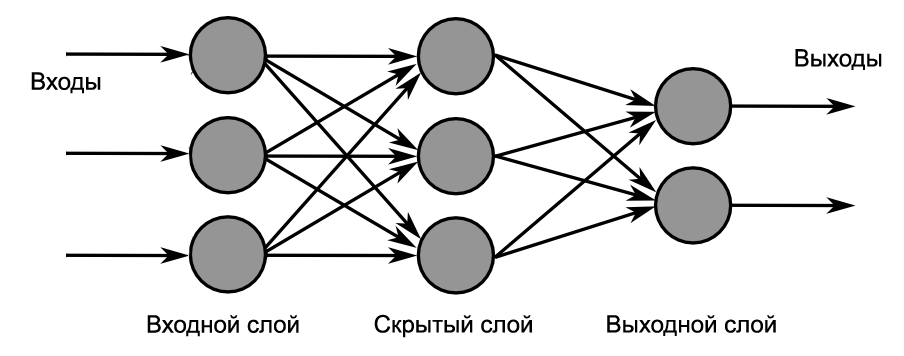
\includegraphics[width=0.8\textwidth]{inc/img/simple-nn.png}
	\caption{Схема простой нейронной сети}
	\label{anal:simple-nn}
\end{figure}

\begin{itemize}
	\item Входной слой -- распределение входных сигналов остальным нейронам. Нейроны этого слоя не производят никаких вычислений.
	\item Скрытый слой -- принимает сигналы с предыдущего слоя, обрабатывает поулченую информацию и передает результат следующему слою.
	\item Выходной слой -- выопляет схожие со скрытым слоем функции за исключением того, что результатом работы выходного слоя является результат работы всей нейронной сети.
\end{itemize}

Каждый слой состоит из нейронов, каждый из которых можно описать математически с помощью его параметров:

\begin{itemize}
	\item Вектор входных данных $X$, состоящий из значений $x_1, ..., x_n$.
	\item Порогове число $b$, является константой, добавляющееся к входному вектору.
	\item Вектор входных весов $W$, состоящий из значений $w_1, ..., w_n$.
	\item Нелинейная активационная функция $\sigma$, которая может быть:
	\begin{itemize}
		\item Гиперболический танцгенс (рис. \ref{anal:th}):
		
		\begin{equation}
			\sigma(x) = \frac{e^x - e^{-x}}{e^x + e^{-x}}
		\end{equation}
		
		\begin{figure}
			\centering
			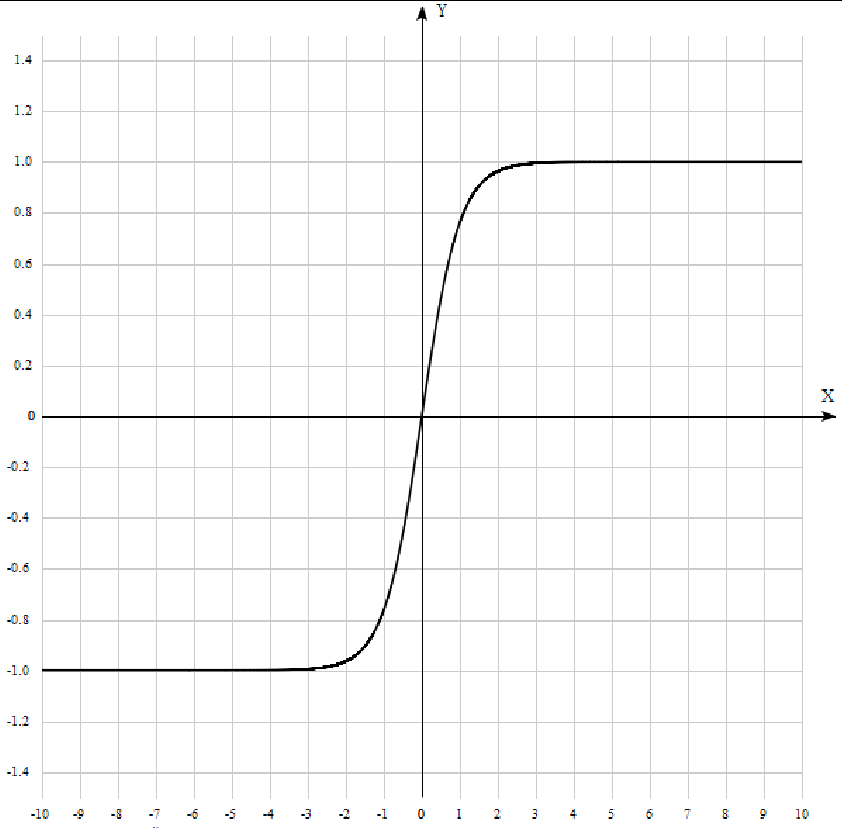
\includegraphics[width=0.5\textwidth]{inc/img/th.png}
			\caption{График гиперболического тангенса}
			\label{anal:th}
		\end{figure}
		
		\item Сигмоида (рис. \ref{anal:sigm}):
		
		\begin{equation}
		\sigma(x)=\frac{1}{1+e^{-x}}
		\end{equation}
		
		\begin{figure}
			\centering
			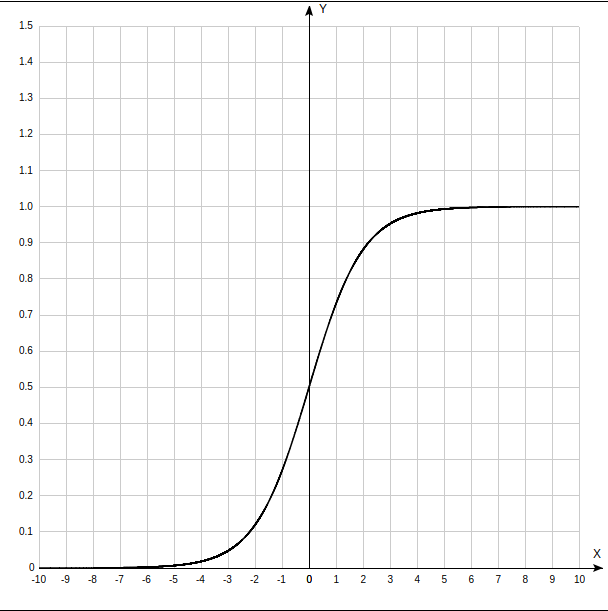
\includegraphics[width=0.5\textwidth]{inc/img/sigmoid.png}
			\caption{График сигмоиды}
			\label{anal:sigm}
		\end{figure}
		
		\item Линейная функция активации ReLU (рис. \ref{anal:relu}):
		
		\begin{equation}
		\sigma(x) = max(0, x)
		\end{equation}
		
%		\begin{figure}
%			\centering
%			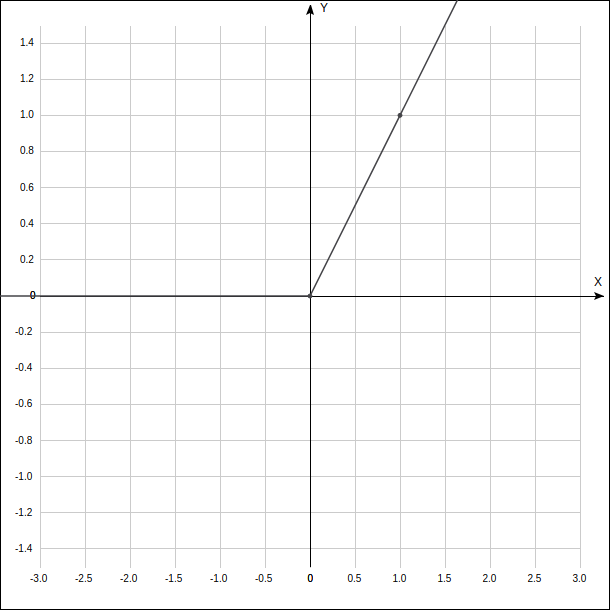
\includegraphics[width=0.5\textwidth]{inc/img/relu.png}
%			\caption{График ReLU}
%			\label{anal:relu}
%		\end{figure}
		
	\end{itemize}
	\item Выходное значение, которое находится по формуле:
	
	\begin{equation}
	a = \sigma( \sum_{i=1}^{n}w_ix_i + b )
	\end{equation}
	
\end{itemize}

Поскольку каждый узел содержит нелинейную функцию, сеть способна изучать различные нелинейные представления входных данных с помощью различных комбинаций входных узлов и функций активации.

\subsubsection{Глубинные нейронные сети}

Глубинные нейронные сети (англ. Deep neural networks) -- нейронные сети с более чем одним скрытым слоем (рис. \ref{anal:DNN}).

\begin{figure}
	\centering
	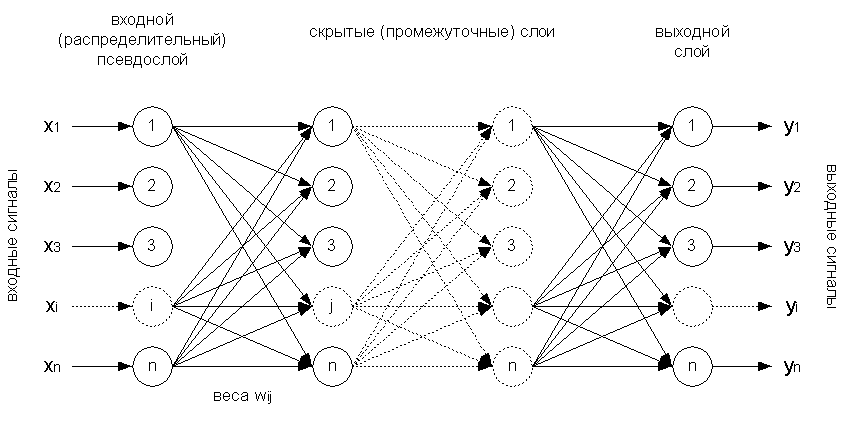
\includegraphics[width=0.8\textwidth]{inc/img/dnn.png}
	\caption{Общая схема ГНС}
	\label{anal:DNN}
\end{figure}

По мере того как данные проходят через более чем один слой, можно обнаружить более абстрактные представления данных, что может помочь улучшить классификацию данных. Каждый слой глубинной сети имеет входы и выходы, и Количество входов каждого слоя зависит от количества выходов его предшественника. Если вход $k-го$ слоя -- $x_k$, то его выход можно записать как:

\begin{equation}
a_k = \sigma_k( b_k + \sum_{i=1}^{n} w_{k,i} x_{k,i} )
\end{equation}

На каждом отдельном слое могут быть использованы отдельные активационные функции.

ГНС рассматривались в качестве инструмента в задачах выделения инструментальных аудио источников\cite{Uhlich}.

Метод состоит из трех основных шагов:

\begin{enumerate}
	\item Препроцессинг
	
	Исходный сигнал $y(n)$ преобразуется в его частотное представление с помощью оконного преобразования Фурье, используя прямоугольную оконную функцию. Из этого представления строится вектор $x \in \Re^{(2C+1)L}$, состоящий из суммы значений магнитуды текущего кадра и $C$ предыдущих/следующих кадров, $L$ -- количество значений магнитуды на кадр.
	
	Полученный вектор нормализуется с помощью числа $\gamma > 0$, являющегося средней Евклидовой нормой $2C+1$ кадоров.
	
	\item Работа глубокой нейронной сети
	
	Полученный нормализованный вектор подается на вход DNN, состоящей из $K$ слоев, с выпрямленной линейной функцией активации (англ. rectified linear unit, ReLU), имеющей вид
	\begin{equation}
	x_{k+1} = max(W_k x_k + b_k , 0), k = 1, ..., K
	\label{anal:relu}
	\end{equation}
	где 
	\begin{itemize}
		\item $x_k$ -- входой вектор для k-го слоя, в частности $x_1$ является исходных вектором, $x_{K+1}$ -- результирующий вектор работы ГНС $\hat s$
		\item $W_k$ -- веса k-го слоя
		\item $b_k$ -- пороговые значения k-го слоя
	\end{itemize}

	Результатом работы ГНС является вектор $\hat s$, являющийся значением магнитудного окна $s \in \Re^L$ выделяемого инструмента.
	
	\item Восстановление
	
	Данный шаг предполагает получение результата применения ОПФ к выделяемому сигналу $s(n)$ при помощи фазы ОПФ исходного сигнала и произведения каждого полученного вектора $\hat{s}$ с коэффициентом нормализации $\gamma$, используемым выше. Получение итогового сигнала происходит с помощью обратного ОПФ.
	
\end{enumerate}

Общая схема работы метода представлена на рисунке \ref{anal:DNN-inst}.

\begin{figure}
	\centering
	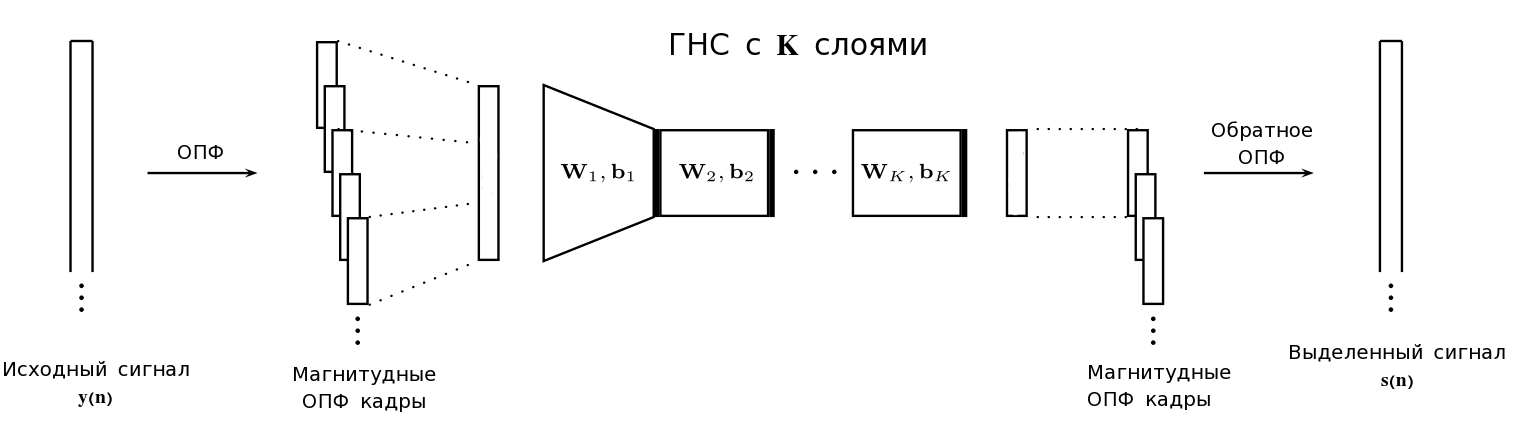
\includegraphics[width=\textwidth]{inc/img/DNN-inst.png}
	\caption{Схема работы метода выделения инструментальных аудио сигналов с использованием ГНС}
	\label{anal:DNN-inst}
\end{figure}

\subsubsection{Сверточные нейронные сети}

Сверточные нейронные сети (англ. Convolutional neural networks) -- это вариант нейронных сетей, вдохновленных зрительной корой головного мозга человека\cite{Hubel}, используются в основном для обработки изображений. СНС используют локальную пространственную корреляцию между входными нейронами из изображения с помощью локальных сенсорных полей. Для иллюстративных целей входной слой вместо одномерного слоя нейронов можно рассматривать как двумерную матрицу, как в случае с файлом изображения. Для изображений значения этой двумерной матрицы представляют интенсивности пикселей. 

В обычной нейронной сети каждый входной нейрон был бы связан с каждый нейроном на первом скрытом слое, в то время как в СНС каждый нейрон первого скрытого слоя связан только с небольшой группой нейронов (рис. \ref{anal:CNN-first}). Сенсорное поле перемещается по всему входному массиву для формирования скрытого слоя. Движение может иметь различный шаг, например на рисунке \ref{anal:CNN-first} изображен шаг (1, 1). Количество нейронов в скрытом слое зависит от количества единиц во входном слое, шага и размера поля.

\begin{figure}
	\centering
	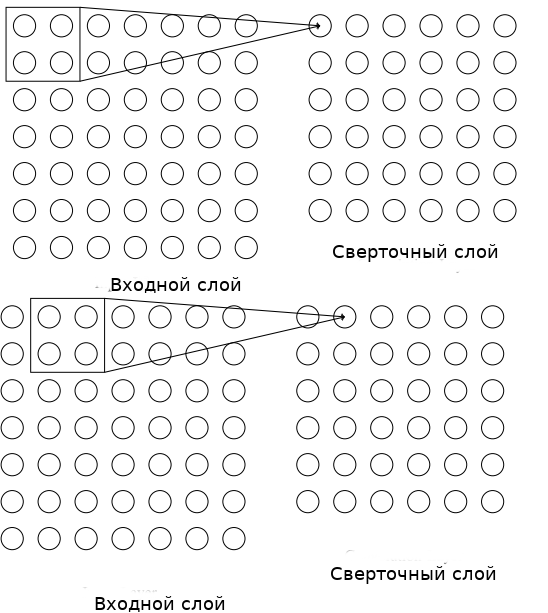
\includegraphics[width=0.6\textwidth]{inc/img/cnn-first.png}
	\caption{Связывание входного слоя с первым скрытым слоем}
	\label{anal:CNN-first}
\end{figure}

Если входной слой имеет размерность $M \times N$, шаг равен (1, 1) и сенсорное поле имеет размерность $A \times B$, то скрытый слой будет иметь размерность $(M - A + 1) \times (N - B + 1)$. Ключевая особенность СНС заключается в том, что нейроны скрытого сверточного слоя разделяют веса и смещения, так что процесс работы сети похож на свертку матрицы размерности $A \times B$ над матрицей $M\times N$.

Результат $j,k-го$ нейрона сверточного слоя математически можно описать как:

\begin{equation}
a_{j,k} = \sigma \Bigg(b + \sum_{l=0}^{A-1} \sum_{m=0}^{B-1} w_{i,m}x_{j+l,k+m}\Bigg)
\end{equation}

Другими словами, сверточный слой вычисляет активацию объекта размерности AxB в разных областях входного слоя. Сопоставление входного слоя с сверточным часто называют векторной картой, а общие веса и единицы смещения называются ядром. Так как каждое из этих ядер идентифицирует одну особенность во входном слое, то сверточный слой обычно включает в себя более одного ядра или карты признаков.

В контексте задачи разделения источников СНС используют для реализации основной идеи ФНМ. В то время, как ФНМ алгоритму необходимо находить базисные вектора для каждой ноты аудиоисточника, рассматриваемый алгоритм использует СНС с целью унификации этих действий через вычесление меньших устойчивых тембральных структур на меньших частях спектограммы. Общая схема работы алгоритма представлена на рисунке \ref{anal:CNN}.

\begin{figure}
	\centering
	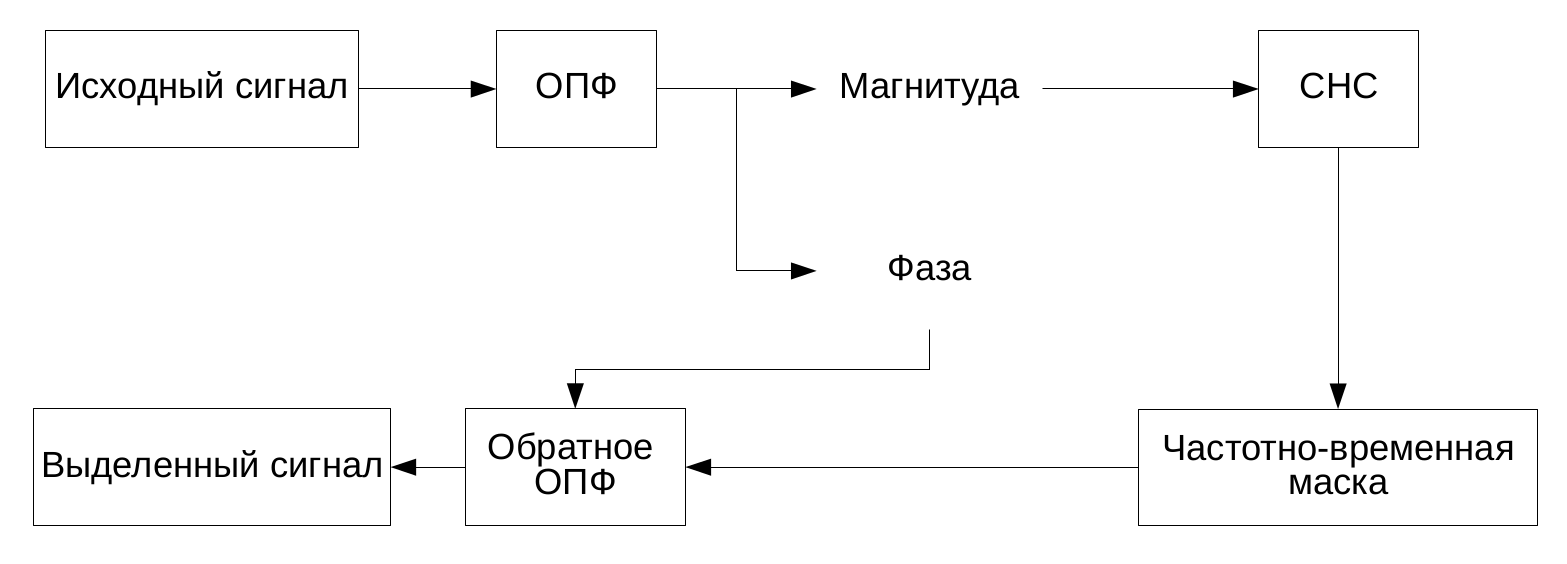
\includegraphics[width=\textwidth]{inc/img/CNN}
	\caption{Схема работы метода выделения аудио сигналов источников с использованием СНС}
	\label{anal:CNN}
\end{figure}

На вход СНС подается магнитудная спектограма, являющаяся результатом применения ОПФ к исходному сигналу. 

Работа нейронной сети происходит в четыре этапа:

\begin{enumerate}
	\item Свертка
	
	Состоит из двух сверточных слоев и объединяющего слоя. 
	\begin{enumerate}
		\item Тембральный сверточный слой: получает локальную информацию о тембре, позволяя модели изучать особенности тембра. В отличие от подхода ФНМ, когда для каждого источника определяются конкретные базисные и активационные вектора, эти характеристики являются общими для отдельных источников.
		\item Объединяющий слой: сжимает информацию, указанную в первом слое по частоте и времени для достижения компактного представления данных. На данном слое сравниваются результаты трех типов: без уплотнения, с уплотнением по частоте и с уплотнением по частоте и времени одновременно.
		\item Временный сверточный слой: изучает различные типы временных изменений для разных инструментов на основании характеристик, полученных из тембрального сверточного слоя. Результатом являются частотно-временные характеристики различных аудио источников. 
	\end{enumerate}
	
	\item Сокращение размерности
	
	Данный слой состоит из нелинейной комбинации признаков, полученных из предыдущих слоев, с ReLU. Слой выбирается таким образом, чтобы иметь меньше элементов для уменьшения общих параметров сети и обеспечения того, чтобы сеть не перегружала данные и могла создавать надежное представление данных.
	
	\item Обратная свертка
	
	Проводятся действия, являющихся обратными операции свертки. Состоит из последовательной развертки и масштабирования данных.
	
	\item Частотно временное экранирование
	
	На данном этапе на основе полученных данных вычисляется частотно-временная маска для каждого выделяемого источника:
	
	\begin{equation}
	m_a t (f) = \frac{|\hat{y}_{at}(f)|}{\sum_{n=1}^{N} |\hat{y}_{nt}(f)|}
	\end{equation}
	
	где $\hat{y}_{nt}(f)$ -- результат работы СНС для $n$-го источника в момент времени $t$, N - число выделяемый источников.
	
	Полученная маска применяется к исходному сигналу, в результате получая спектрограмму выделяемого сигнала:
	\begin{equation}
	y_n(f) = m_n t(f)x_t(f)
	\end{equation}
	
	где $x_t(f)$ -- спектрограмма исходного сигнала.
	
\end{enumerate}

Как и в случае с ГНС, для вычисления выделяемого сигнала, к полученной спектрограмме применяется обратное ОПФ.

\subsubsection{Рекуррентные нейронные сети}

Поскольку аудио сигналы имеют временной контекст, нейронной сети должна быть предоставлена некоторая память для добавления контекстной информации из прошлого. Одним из решений является использование рекуррентной нейронной сети. Суть заключается в соединении скрытого слоя с самим собой (рисунок \ref{anal:rnn}). То есть вход слоя в момент времени t можно описать так:

\begin{equation}
J(j,t) = \sum X(i,t) W_1(i,j) + b_1 W_1(i+1, j) + W_2 H( J(j, t-1) )
\end{equation}

где $H(J(j,t-1))$ -- выход слоя в момент времени $t-1$. 

\begin{figure}
	\centering
	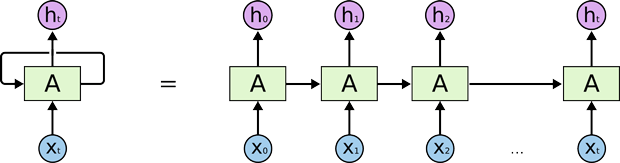
\includegraphics[width=\textwidth]{inc/img/rnn-simple.png}
	\caption{Схема однойслойной рекуррентной нейронной сети}
	\label{anal:rnn}
\end{figure}

Существуют так же многослойные рекуррентные сети. Различают многослойные РНС с одной рекуррентной связью на l-слое и сложенные многослойные РНС, с рекуррентными связями на каждом скрытом слое (рисунок \ref{anal:drnn}).

\begin{figure}
	\centering
	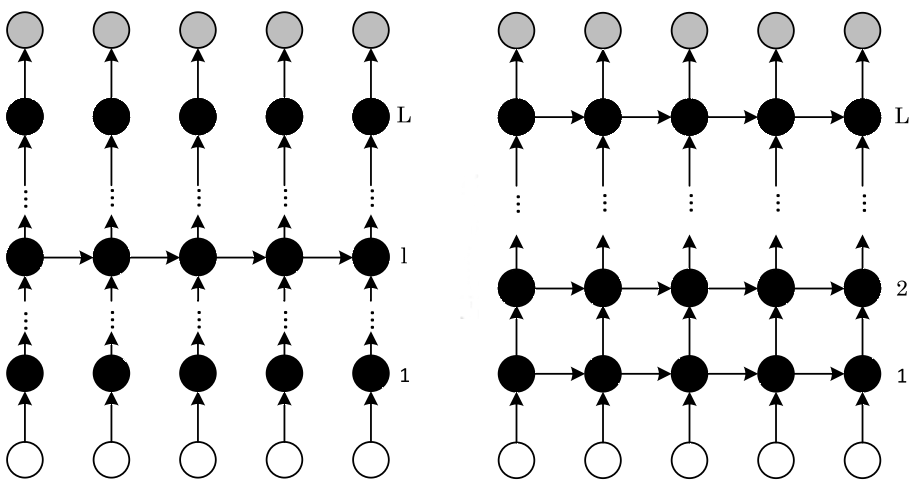
\includegraphics[width=\textwidth]{inc/img/rdnn.png}
	\caption{Схемы многослойной РНС с одной рекуррентной связью и сложенной многослойной РНС, с L скрытыми слоями}
	\label{anal:drnn}
\end{figure}

Эта работа будет сфокусирована на использовании сложенной многослойной РНС. На вход сети будет подаваться спектрограмма исходного сигнала, полученная из ОПФ. Сеть должна генерировать частотно-временную маску, которая на последнем слое будет применяться к спектрограмме исходного слоя.

\section{Оценка методов выделения источников}

Оценка методов выделения источников является нетривиальной задачей, учитывая субъективность мнения о качестве аудио записи. Тем не менее, оценочные метрики были изучены и формализованы группой исследователей во главе с Имануилом Винсентом\cite{Vincent}.
Оценка метода выделения аудио источника должна проходить в контексте приложения. Исходный сигнал представляется линейной комбинацией сигналов источников $(s_j)_{j\in J}$ с добавлением шума. Простейшей мерой является норма L2, выражающаяся в разнице между полученным источником $\hat{s}_j$ и ожидаемым источником $s_j$:

\begin{equation}
D = \min_{\epsilon=\pm 1} \Bigg | \Bigg | \frac{\hat{s}_j}{||\hat{s}_j||} - \epsilon \frac{s_j}{||s_j||} \Bigg | \Bigg |^2
\end{equation}

Данная разность всегда неотрицательна и равна нулю только в случае $\hat{s}_j = s_j$. В худшем случае, когда вектора $\hat{s}_j$ и $\hat{s}$ ортогональны, разность останется ограниченной максимумом двух, так как источники нормализованы. Так же, в случае шумов или других искажений, которые добавляются к искомым источниками, данная мера будет имет низкое значение, которое может быть нежелательным, в зависимости от приложения. Например, при обработке аудиозаписей высокого качества, такие шумы могут быть нежелательными, а в случае, когда к выделяемым источникам планируется применять дополнительную, данными искажениями можно пренебречь.

Для учета этих случаем искомый источник разделяется на четыре части:

\begin{equation}
\hat{s}_j = s_{target} + e_{interf} + e_{spat} + e_{artif}
\label{anal:source}
\end{equation}

где

\begin{itemize}
	\item $s_{targer}$ -- модификация целевого источника, которая может содержать определенные допустимые искажения, $F$;
	\item $e_{interf}$ -- помехи, полученные от нежелательных источников $(s_{j'})_{j' \neq j}$;
	\item $e_{spat}$ -- пространственные искажения;
	\item $e_{artif}$ -- остальные виды шумов, не входящие в $F$ и другие артефакты.
\end{itemize}

Для определения метрик используются ортогональные проекции, которые могут быть определены следующим образом: для подпространства с векторами $y_1, y_2, ... , y_n$, $\prod{y_1, y_2, ... , y_n}$ -- матрица, проектирующая вектора в данное подпространство. Определяются следующие матрицы:

\begin{equation}
P_{s,j} = \prod(s_j)
\end{equation}

\begin{equation}
P_{S} = \prod\{(s_{j'})_{1\le j' \le n}\}
\end{equation}

\begin{equation}
P_{S, n} = \prod\{(s_{j'})_{1\le j' \le n}, (n_i)_{1 \le i \le m} \}
\end{equation}

С помощью этих проецирующих матриц слагаемые из формулы \ref{anal:source} можно представить следующим образом:

\begin{equation}
	s_{target} = P_{s,j} \hat{s}_j
\end{equation}

\begin{equation}
e_{interf} = P_{S} \hat{s}_j - P_{s,j} \hat{s}_j
\end{equation}

\begin{equation}
e_{spat} = P_{S, n} \hat{s}_j - P_{s,j} \hat{s}_j
\end{equation}

\begin{equation}
e_{artif} = \hat{s}_j - P_{S, n} \hat{s}_j
\end{equation}

Для вычисления $s_{target}$ используется скалярное произведение:

\begin{equation}
s_{target} = (\hat{s}_j, s_j) \frac{s_j}{|| s_j ||^2}
\end{equation}

Для вычесления $P_S$ и $P_{S,n}$ используется вектор коэффициентов $c$:

\begin{equation}
c = R_{SS}^{-1}[ (\hat{s}_j, s_1) ... (\hat{s}_j, s_n) ]^H
\end{equation}

где $R_{SS}$ -- определитель Грама (грамиан). $P_S \hat{s}_j$ можно записать как:

\begin{equation}
P_S \hat{s}_j = c^H s
\end{equation}

где $(.)^H$ -- Эрмитовская перестановка. 

Если источник и шумовой сигнал взаимно ортогональны, то можно записать:

\begin{equation}
	e_{interf} = \sum_{j' \ne j} (\hat{s}_j, s_{j'}) \frac{s_{j'}}{|| s_{j'} ||^2}
\end{equation}

\begin{equation}
P_{S,n}\hat{s}_j = P_S \hat{s}_j + \sum_{i=1}^{m}(\hat{s}_j, n_i) \frac{n_i}{|| n_i ||^2}
\end{equation}

На основании этих значений можно записать следующие метрики:

\begin{enumerate}
	\item Отношение источника к искажению:
	
	\begin{equation}
		SDR = 10 \log_{10} \frac{|| s_{target} ||^2}{|| e_{interf} + e_{spat} + e_{artif} ||^2}
	\end{equation}
	
	Эта мера оценивает общую эффективность алгоритма разделения источников
	
	\item  Отношение источника к интерференции:
	
	\begin{equation}
		SIR = 10 \log_{10} \frac{|| s_{target} ||^2}{|| e_{interf} ||^2}
	\end{equation}
	
	Эта мера отражает подавление помех во время выделения.
	
	\item Отношение образа к пространственному искажению:
	
	\begin{equation}
	ISR = 10 \log_{10} \frac{|| s_{target} + e_{interf} ||^2}{|| e_{spat} ||^2}
	\end{equation}
	
	\item Отношение источника к артефактам:
	
	\begin{equation}
	SAR = 10 \log_{10} \frac{|| s_{target} + e_{interf} + e_{spat} ||^2}{|| e_{artif} ||^2}
	\end{equation}
	
	Эта мера оценивает артефакты, получаемые во время разделения источников.
\end{enumerate}

Значение компонент $s_{target}, e_{interf}, e_{spat}$ и $e_{artif}$ изменяются во времени. Предлагается разделять сигнал на части для вычисления локальных значений. Итоговые значения могут быть суммированы с использованием статистических мер.

\section{Сравнение методов}

Метод главных компонент и Факторизация неотрицательных матриц не участвуют в сравнении, так как являются строго статистическими методами и требуют дополнительных действий для подбора начальных значений для каждого конкретного примера.

\begin{table}[h]
	\caption{\label{tab:canonsummary}Сравнение алгоритмов выделения источников}
	\begin{center}
		\begin{tabular}{|c|c|c|c|}
			\hline
			Метод & Метрика & Вокал & Аккомпанемент \\
			\hline
			CNN & SDR & -0.6 ± 4.9 & 4.5 ± 1.2 \\
				& SIR & 1.9 ± 6.2 & 14.9 ± 5.6 \\
				& SAR & 3.6 ± 2.1 & 16.4 ± 2.9 \\
				& ISR & 7.3 ± 2.7 & 6.9 ± 1.0 \\
			\hline
			DNN & SDR & -8.9 ± 4.4 & 4.1 ± 2.6 \\
			& SIR & 10.8 ± 3.1 & 10.7 ± 3.8 \\
			& SAR & -6.6 ± 4.6 & 12.1 ± 3.9 \\
			& ISR & 4.8 ± 2.8 & 5.0 ± 3.0 \\
			\hline
			FASST & SDR & -1.8 ± 5.8 & 8.9 ± 3.2 \\
			& SIR & -3.7 ± 7.5 & 13.7 ± 3.0 \\
			& SAR & 4.3 ± 1.4 & 13.1 ± 3.2 \\
			& ISR & 5.6 ± 2.5 & 13.5 ± 2.5 \\
			\hline
		\end{tabular}
	\end{center}
\end{table} 

Значение метрик получено на наборе данных DSD100 \cite{DSD100}. Как видно из таблицы, использование нейронных сетей дает лучший результат в задаче выделения аудио источников.

\section{Вывод}

Необходимо разработать и реализовать метод выделения голосовой составляющей из монофонического аудио сигнала на основе многослойной РНС.

Для выполнения работы необходимо спроектировать и реализовать продукт, осуществляющий автоматизированное выделение вокальной составляющей из музыкального аудио сигнала. На вход программному продукту подаются одноканальные музыкальные произведения в формате WAVE. На выходе программный продукт генерирует два одноканальных WAVE-файла, содержащие вокальный аудио сигнал и аккомпанемент. Исходные музыкальные произведения должны представлять из себя песни с эстрадным стилем вокала. Разделяемые записи должны представлять собой записи <<без потерь>>, на них не должно быть шумов. Для более точного разделения запись должна быть без фильтров, применяемых на этапе пост-обработки.

Для определения качества выделения источников будут использоваться сравнение полученных в результате работы алгоритмов данных с заранее известными на основе описанных выше метрик.

Так же необходимо сравнить показатели разработанного метода с значениями, описанными в таблице \ref{tab:canonsummary}.

%%% Local Variables:
%%% mode: latex
%%% TeX-master: "rpz"
%%% End:
